\section{Noise Generation}
\label{section:noise-generation}
Nature's unpredictability plays a big role in the diversity and appearance of cloudscapes. In shaders, an approach to that \textit{randomness} is used called \textit{\gls{noisegeneration}}.
In order to be able to implement random \gls{noisegeneration}, several important topics need to be looked into. It is best to start with randomness in computer science and how it is handled inside a shader program.

\subsection{Random Numbers}
Unfortunately, there is no magic function which returns a pure random number inside the seemingly predictable and rigid code environment.
So the question arises as to how such randomness can be generated.
\\
For this, the function $rnd(x) = fract(sin(x))$ is inspected, where $fract(x) = x - floor(x)$.

\begin{figure}[H]
    \centering
    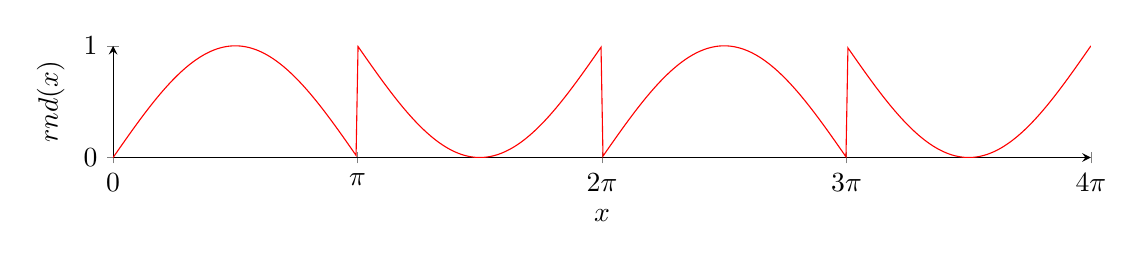
\begin{tikzpicture}[scale=1.0]
        \begin{axis}[
            samples=500,
            domain=0:4*pi,
            axis lines=left,
            xlabel=$x$,
            ylabel={$rnd(x)$},
            height=3cm,
            width=14cm,
            ytick={0,1},
            xtick={0,pi,2*pi,3*pi,4*pi},
            xticklabels={$0$,$\pi$,$2\pi$,$3\pi$,$4\pi$}
            ]
        \addplot[red] plot (\x, { sin(\x*1 r) - floor(sin(\x*1 r)) });
        \end{axis}
    \end{tikzpicture}
    \captionof{figure}{Random numbers with the fractional value of sine of x.}
\end{figure}

\noindent
The sine values fluctuate between $-1.0$ and $1.0$, but with $fract$, only the fractional part is evaluated, turning the negative values into positive ones.
This effect can be used to get some pseudo-random values by "compressing" the function horizontally, or in other words by increasing the frequency of the sine wave.
\\
The next figure displays the function $rnd(x) = fract(sin(x) * 10000)$.

\begin{figure}[H]
    \centering
    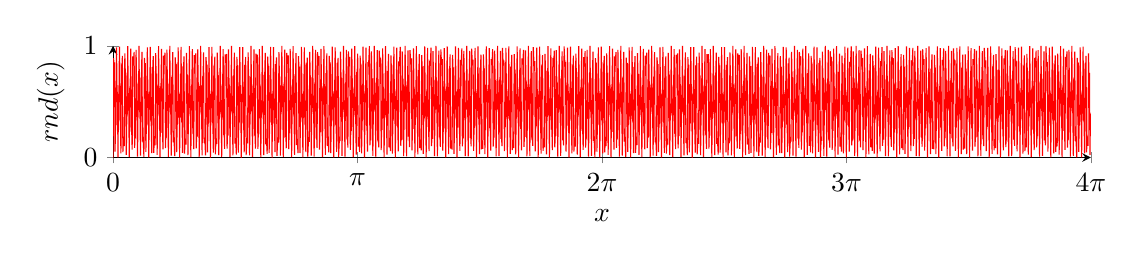
\begin{tikzpicture}[scale=1.0]
        \begin{axis}[
            samples=2000,
            domain=0:4*pi,
            axis lines=left,
            xlabel=$x$,
            ylabel={$rnd(x)$},
            height=3cm,
            width=14cm,
            ytick={0,1},
            xtick={0,pi,2*pi,3*pi,4*pi},
            xticklabels={$0$,$\pi$,$2\pi$,$3\pi$,$4\pi$},
            ]
        \addplot[red] plot (\x, { sin(\x*10000) - floor(sin(\x*10000)) });
        \end{axis}
    \end{tikzpicture}
    \captionof{figure}{Random numbers with the fractional value of sine of x multiplied by 10000.}
\end{figure}

\noindent
It is clearly visible that the function $rnd(x)$ became chaotic and returns practically random values. However, it is noteworthy that $rnd(x)$ is still a deterministic function, which means for example $rnd(1.0)$ is always going to return the same value.

\clearpage
\subsection{2D Random}
To generate a pseudo-random number from two and three values instead of one, the same function can be used, with some tweaks. Those two numbers come as a two-dimensional vector, which needs to be transformed into a single floating point number.
According to Vivo, the dot product is particularily helpful in that case \cite{online:thebookofshaders}. It returns a single float value between $0.0$ and $1.0$ depending on the alignment of two vectors.
They describe the following methods:

\begin{lstlisting}[language=HLSL, caption=Implementation of 2D random number generation., label=lst:random:2d]
float random(float2 co) {
    float2 other = float2(12.9898, 78.233);
    return fract(sin(dot(co, other)) * 43758.5453123);
}
\end{lstlisting}

\begin{lstlisting}[language=HLSL, caption=Implementation of 3D random number generation., label=lst:random:3d]
float random(float3 co) {
    float3 other = float3(12.9898, 78.233, 37.719);
    return fract(sin(dot(co, other)) * 43758.5453123);
}
\end{lstlisting}

\noindent
When using the fragment coordinates as the vector \lstinline[language=HLSL]{co} to call \lstinline[language=HLSL]{random(co)} for every pixels, the resulting image shows a seemingly random assortment of pixels holding values from 0 to 1 (from black to white).

\begin{figure}[H]
    \centering
            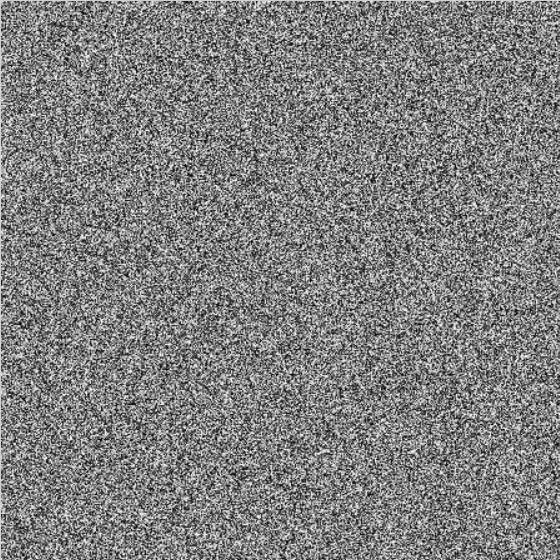
\includegraphics[width=0.45\linewidth]{noise/2d random}
            \captionof{figure}{2D random function visualized.}
            \label{img:noise:2d:random}
\end{figure}

\noindent
This method of procedural randomness still has one major flaw: It has no patterns. Contratictory to the word \textit{random}, a certain pattern is required in order to generate \textit{random} clouds. Luckily, there is more to random generation than just a highly sped up sine wave.

\clearpage
\subsection{Procedural Noise Patterns}
Now that the concept of random numbers in the world of shaders is no longer a mystery, more advanced noise generation algorithms can be introduced.
When using the word \textit{\gls{noise}} in this context, usually procedural pattern generation is meant.

\subsubsection{Perlin Noise}
One of the most commonly used procedural pattern generation algorithms is that of Ken Perlin. Named after him, the algorithm works with the gradient, which was already introduced in \sectionref{section:rendering:surfacenormalestimation}.
\\
It consists of the following three steps: 
\begin{enumerate}
    \item grid definition
    \item dot product calculation between random gradient and distance vectors
    \item interpolation of those dot product values
\end{enumerate}

\noindent
Note that the following example refers to two-dimensional perlin noise generation, but with some tweaks, is very much applicable for higher dimensional noise generation.
\\
First, the 2D image space is split into a grid. For each vertex or corner point on this grid, a pseudo-random gradient vector is determined.

\begin{figure}[H]
    \centering
        \begin{minipage}{0.47\linewidth}
            \begin{tikzpicture}[scale=0.8, x=2cm,y=2cm]
                \tikzset{c/.style = {shorten <=-4pt, shorten >=-4pt}}
                \tikzset{smalledge/.style = {-{Latex[length=2mm]},shorten <=-4pt}}
              
                \node (x1y1) at (0,0) {\textbullet};
                \node (x2y1) at (1,0) {\textbullet};
                \node (x3y1) at (2,0) {\textbullet};
                \node (x4y1) at (3,0) {\textbullet};
        
                \node (x1y2) at (0,1) {\textbullet};
                \node (x2y2) at (1,1) {\textbullet};
                \node (x3y2) at (2,1) {\textbullet};
                \node (x4y2) at (3,1) {\textbullet};
        
                \node (x1y3) at (0,2) {\textbullet};
                \node (x2y3) at (1,2) {\textbullet};
                \node (x3y3) at (2,2) {\textbullet};
                \node (x4y3) at (3,2) {\textbullet};
        
                \node (x1y4) at (0,3) {\textbullet};
                \node (x2y4) at (1,3) {\textbullet};
                \node (x3y4) at (2,3) {\textbullet};
                \node (x4y4) at (3,3) {\textbullet};
        
                \draw[c] (x1y1) edge node{} (x4y1);
                \draw[c] (x1y2) edge node{} (x4y2);
                \draw[c] (x1y3) edge node{} (x4y3);
                \draw[c] (x1y4) edge node{} (x4y4);
        
                \draw[c] (x1y1) edge node{} (x1y4);
                \draw[c] (x2y1) edge node{} (x2y4);
                \draw[c] (x3y1) edge node{} (x3y4);
                \draw[c] (x4y1) edge node{} (x4y4);
        
                % arrows
                \draw[smalledge, red] (x1y1) edge node{} ($ (x1y1) + (-0.6,0.2) $);
                \draw[smalledge, red] (x2y1) edge node{} ($ (x2y1) + (0.4,0.4) $);
                \draw[smalledge, red] (x3y1) edge node{} ($ (x3y1) + (0.3,-0.5) $);
                \draw[smalledge, red] (x4y1) edge node{} ($ (x4y1) + (0.5,-0.3) $);
        
                \draw[smalledge, red] (x1y2) edge node{} ($ (x1y2) + (0.3,-0.5) $);
                \draw[smalledge, red] (x2y2) edge node{} ($ (x2y2) + (0.2,0.6) $);
                \draw[smalledge, red] (x3y2) edge node{} ($ (x3y2) + (0.6,-0.2) $);
                \draw[smalledge, red] (x4y2) edge node{} ($ (x4y2) + (0.3,-0.5) $);
        
                \draw[smalledge, red] (x1y3) edge node{} ($ (x1y3) + (-0.3,0.5) $);
                \draw[smalledge, red] (x2y3) edge node{} ($ (x2y3) + (-0.3,-0.5) $);
                \draw[smalledge, red] (x3y3) edge node{} ($ (x3y3) + (0.5,-0.3) $);
                \draw[smalledge, red] (x4y3) edge node{} ($ (x4y3) + (0.5,0.3) $);
        
                \draw[smalledge, red] (x1y4) edge node{} ($ (x1y4) + (0.3,0.5) $);
                \draw[smalledge, red] (x2y4) edge node{} ($ (x2y4) + (-0.1,-0.7) $);
                \draw[smalledge, red] (x3y4) edge node{} ($ (x3y4) + (-0.4,0.4) $);
                \draw[smalledge, red] (x4y4) edge node{} ($ (x4y4) + (-0.3,0.5) $);
        
                \end{tikzpicture}
                \captionof{figure}{Perlin grid with pseudo-random gradient vectors.}
                \label{img:tikz:noise:perlin:gradient}
        \end{minipage}
    \hfill
    \begin{minipage}{0.47\linewidth}
        \begin{tikzpicture}[scale=0.8, x=2cm,y=2cm]
            \tikzset{c/.style = {shorten <=-4pt, shorten >=-4pt}}
            \tikzset{smalledge/.style = {-{Latex[length=2mm]},shorten <=-4pt}}

            \begin{scope}
                \clip (0,0) rectangle (3,3);
                
                \node [shading=axis,rectangle,left color=white, right color=gray,shading angle=180+65,  minimum width=0.8*2cm, minimum height=0.8*2cm] (box) at (x1y1){};
                \node [shading=axis,rectangle,left color=white, right color=gray,shading angle=180-40,  minimum width=0.8*2cm, minimum height=0.8*2cm] (box) at (x2y1){};
                \node [shading=axis,rectangle,left color=white, right color=gray,shading angle=180-145, minimum width=0.8*2cm, minimum height=0.8*2cm] (box) at (x3y1){};
                \node [shading=axis,rectangle,left color=white, right color=gray,shading angle=180-110, minimum width=0.8*2cm, minimum height=0.8*2cm] (box) at (x4y1){};
                
                \node [shading=axis,rectangle,left color=white, right color=gray,shading angle=180-145, minimum width=0.8*2cm, minimum height=0.8*2cm] (box) at (x1y2){};
                \node [shading=axis,rectangle,left color=white, right color=gray,shading angle=180-10,  minimum width=0.8*2cm, minimum height=0.8*2cm] (box) at (x2y2){};
                \node [shading=axis,rectangle,left color=white, right color=gray,shading angle=180-100, minimum width=0.8*2cm, minimum height=0.8*2cm] (box) at (x3y2){};
                \node [shading=axis,rectangle,left color=white, right color=gray,shading angle=180-165, minimum width=0.8*2cm, minimum height=0.8*2cm] (box) at (x4y2){};
                
                \node [shading=axis,rectangle,left color=white, right color=gray,shading angle=180+30,  minimum width=0.8*2cm, minimum height=0.8*2cm] (box) at (x1y3){};
                \node [shading=axis,rectangle,left color=white, right color=gray,shading angle=180+140, minimum width=0.8*2cm, minimum height=0.8*2cm] (box) at (x2y3){};
                \node [shading=axis,rectangle,left color=white, right color=gray,shading angle=180-120, minimum width=0.8*2cm, minimum height=0.8*2cm] (box) at (x3y3){};
                \node [shading=axis,rectangle,left color=white, right color=gray,shading angle=180-55,  minimum width=0.8*2cm, minimum height=0.8*2cm] (box) at (x4y3){};

                \node [shading=axis,rectangle,left color=white, right color=gray,shading angle=180-30,  minimum width=0.8*2cm, minimum height=0.8*2cm] (box) at (x1y4){};
                \node [shading=axis,rectangle,left color=white, right color=gray,shading angle=180+175, minimum width=0.8*2cm, minimum height=0.8*2cm] (box) at (x2y4){};
                \node [shading=axis,rectangle,left color=white, right color=gray,shading angle=180+45,  minimum width=0.8*2cm, minimum height=0.8*2cm] (box) at (x3y4){};
                \node [shading=axis,rectangle,left color=white, right color=gray,shading angle=180+35,  minimum width=0.8*2cm, minimum height=0.8*2cm] (box) at (x4y4){};
            \end{scope}

            \node (x1y1) at (0,0) {\textbullet};
            \node (x2y1) at (1,0) {\textbullet};
            \node (x3y1) at (2,0) {\textbullet};
            \node (x4y1) at (3,0) {\textbullet};
    
            \node (x1y2) at (0,1) {\textbullet};
            \node (x2y2) at (1,1) {\textbullet};
            \node (x3y2) at (2,1) {\textbullet};
            \node (x4y2) at (3,1) {\textbullet};
    
            \node (x1y3) at (0,2) {\textbullet};
            \node (x2y3) at (1,2) {\textbullet};
            \node (x3y3) at (2,2) {\textbullet};
            \node (x4y3) at (3,2) {\textbullet};
    
            \node (x1y4) at (0,3) {\textbullet};
            \node (x2y4) at (1,3) {\textbullet};
            \node (x3y4) at (2,3) {\textbullet};
            \node (x4y4) at (3,3) {\textbullet};
    
            \draw[c] (x1y1) edge node{} (x4y1);
            \draw[c] (x1y2) edge node{} (x4y2);
            \draw[c] (x1y3) edge node{} (x4y3);
            \draw[c] (x1y4) edge node{} (x4y4);
    
            \draw[c] (x1y1) edge node{} (x1y4);
            \draw[c] (x2y1) edge node{} (x2y4);
            \draw[c] (x3y1) edge node{} (x3y4);
            \draw[c] (x4y1) edge node{} (x4y4);
    
            % arrows
            \draw[smalledge, red] (x1y1) edge node{} ($ (x1y1) + (-0.6, 0.2) $);
            \draw[smalledge, red] (x2y1) edge node{} ($ (x2y1) + (0.4,  0.4) $);
            \draw[smalledge, red] (x3y1) edge node{} ($ (x3y1) + (0.3, -0.5) $);
            \draw[smalledge, red] (x4y1) edge node{} ($ (x4y1) + (0.5, -0.3) $);
    
            \draw[smalledge, red] (x1y2) edge node{} ($ (x1y2) + (0.3, -0.5) $);
            \draw[smalledge, red] (x2y2) edge node{} ($ (x2y2) + (0.2,  0.6) $);
            \draw[smalledge, red] (x3y2) edge node{} ($ (x3y2) + (0.6, -0.2) $);
            \draw[smalledge, red] (x4y2) edge node{} ($ (x4y2) + (0.3, -0.5) $);
    
            \draw[smalledge, red] (x1y3) edge node{} ($ (x1y3) + (-0.3, 0.5) $);
            \draw[smalledge, red] (x2y3) edge node{} ($ (x2y3) + (-0.3,-0.5) $);
            \draw[smalledge, red] (x3y3) edge node{} ($ (x3y3) + (0.5, -0.3) $);
            \draw[smalledge, red] (x4y3) edge node{} ($ (x4y3) + (0.5,  0.3) $);
    
            \draw[smalledge, red] (x1y4) edge node{} ($ (x1y4) + (0.3,  0.5) $);
            \draw[smalledge, red] (x2y4) edge node{} ($ (x2y4) + (-0.1,-0.7) $);
            \draw[smalledge, red] (x3y4) edge node{} ($ (x3y4) + (-0.4, 0.4) $);
            \draw[smalledge, red] (x4y4) edge node{} ($ (x4y4) + (-0.3, 0.5) $);
    
            \end{tikzpicture}
            \captionof{figure}{Perlin grid with visualized gradient vectors.}
            \label{img:tikz:noise:perlin:gradient_visualized}
    \end{minipage}
\end{figure}

\clearpage
\noindent
For the next step, it is easier to only inspect a single cell. Given the algorithm currently processes the highlighted pixel $p$ in \autoref{img:tikz:noise:perlin:singlecell}, the next task is to determine the distance vectors from each adjacent corner point to the that pixel.
Note that in $\mathbb{R}^2$, the amount of corners is four, while in $\mathbb{R}^3$, its eight.

\begin{figure}[H]
    \centering
    \begin{minipage}{0.47\linewidth}
        \begin{tikzpicture}[scale=2, x=2cm,y=2cm]
            \tikzset{c/.style = {shorten <=-4pt, shorten >=-4pt}}
            \tikzset{smalledge/.style = {-{Latex[length=2mm]},shorten <=-4pt}}
            
            \node (x1y1) at (0,0) {\textbullet};
            \node (x2y1) at (1,0) {\textbullet};
            \node (x1y2) at (0,1) {\textbullet};
            \node (x2y2) at (1,1) {\textbullet};
    
            \draw[c] (x1y1) edge node{} (x1y2);
            \draw[c] (x1y1) edge node{} (x2y1);
            \draw[c] (x2y2) edge node{} (x2y1);
            \draw[c] (x2y2) edge node{} (x1y2);
    
            \node[cyan] (pixel) at (0.7,0.6) {\textbullet};
            \draw[c, cyan] (pixel) -- (1.1,0.8) -- (1.3,0.8) node[xshift=-0.4cm,above]{pixel $p$};
    
            % arrows
            \draw[smalledge, red] (x1y1) edge node{} ($ (x1y1) + (-0.45,0.15) $);
            \draw[smalledge, red] (x2y1) edge node{} ($ (x2y1) + (0.3,0.3) $);
            \draw[smalledge, red] (x1y2) edge node{} ($ (x1y2) + (0.225,-0.375) $);
            \draw[smalledge, red] (x2y2) edge node{} ($ (x2y2) + (0.15,0.45) $);
    
        \end{tikzpicture}
        \captionof{figure}{Perlin grid cell with gradient vectors.}
        \label{img:tikz:noise:perlin:singlecell}
    \end{minipage}
    \hfill
    \begin{minipage}{0.47\linewidth}
        \begin{tikzpicture}[scale=2, x=2cm,y=2cm]
            \tikzset{c/.style = {shorten <=-4pt, shorten >=-4pt}}
            \tikzset{smalledge/.style = {-{Latex[length=2mm]},shorten <=-4pt}}
            
            \node (x1y1) at (0,0) {\textbullet};
            \node (x2y1) at (1,0) {\textbullet};
            \node (x1y2) at (0,1) {\textbullet};
            \node (x2y2) at (1,1) {\textbullet};
    
            \draw[c] (x1y1) edge node{} (x1y2);
            \draw[c] (x1y1) edge node{} (x2y1);
            \draw[c] (x2y2) edge node{} (x2y1);
            \draw[c] (x2y2) edge node{} (x1y2);
    
            \node[cyan] (pixel) at (0.7,0.6) {\textbullet};
    
            % arrows
            \draw[smalledge, red] (x1y1) edge node[above]{$\overrightarrow{g_1}$} ($ (x1y1) + (-0.45,0.15) $);
            \draw[smalledge, red] (x2y1) edge node[above]{$\overrightarrow{g_2}$} ($ (x2y1) + (0.3,0.3) $);
            \draw[smalledge, red] (x1y2) edge node[left] {$\overrightarrow{g_3}$} ($ (x1y2) + (0.225,-0.375) $);
            \draw[smalledge, red] (x2y2) edge node[left] {$\overrightarrow{g_4}$} ($ (x2y2) + (0.15,0.45) $);

            % distance vectors
            \draw[smalledge, cyan, shorten >=-4pt] (x1y1) edge node[above]{$\overrightarrow{d_1}$} (pixel);
            \draw[smalledge, cyan, shorten >=-4pt] (x2y1) edge node[left] {$\overrightarrow{d_2}$} (pixel);
            \draw[smalledge, cyan, shorten >=-4pt] (x1y2) edge node[above]{$\overrightarrow{d_3}$} (pixel);
            \draw[smalledge, cyan, shorten >=-4pt] (x2y2) edge node[left] {$\overrightarrow{d_4}$} (pixel);
    
        \end{tikzpicture}
        \captionof{figure}{Perlin grid cell with distance vectors from each vertex to the pixel.}
        \label{img:tikz:noise:perlin:distancevectors}
    \end{minipage}
\end{figure}

\noindent
Then, the dot product is calculated for each distance vector and its gradient vector. This qualifies how similar those two vectors are, returning a positive number if they face the same direction and a negative one for the opposite. The dot product is 0 if the vectors are perpendicular.
$$ 
\begin{array}{l}
    s = g_1 * d_1,\\
    t = g_2 * d_2,\\
    u = g_3 * d_3,\\
    v = g_4 * d_4.
\end{array}
$$

\noindent
The values $s, t, u, v$ represent the influences of the respective gradient on the final color of the pixel $p$. 
When visualizing those values as vectors with their length being the influence, it looks like this:
\begin{figure}[H]
    \centering
    \begin{tikzpicture}[scale=2, x=2cm,y=2cm]
        \tikzset{c/.style = {shorten <=-6pt, shorten >=-6pt}}
        \tikzset{smalledge/.style = {-{Latex[length=2mm]},shorten <=-6pt}}
        
        \node (x1y1) at (0,0) {\textbullet};
        \node (x2y1) at (1,0) {\textbullet};
        \node (x1y2) at (0.6,0.4) {\textbullet};
        \node (x2y2) at (1.6,0.4) {\textbullet};

        \node[above] at (x1y1) {$S$};
        \node[below] at (x2y1) {$T$};
        \node[below] at (x1y2) {$U$};
        \node[above] at (x2y2) {$V$};

        \draw[c] (x1y1) -- (x1y2);
        \draw[c] (x1y2) -- (x2y2);
        \draw[c] (x2y2) -- (x2y1);
        \draw[c] (x2y1) -- (x1y1);

        % arrows
        \draw[smalledge, red] (x1y1) edge node[left]{$s$} ($(x1y1) + (0,-0.225)$);
        \draw[smalledge, red] (x2y1) edge node[left]{$t$} ($(x2y1) + (0,0.1)$);
        \draw[smalledge, red] (x1y2) edge node[left]{$u$} ($(x1y2) + (0,0.3075)$);
        \draw[smalledge, red] (x2y2) edge node[left]{$v$} ($(x2y2) + (0,-0.225)$);

    \end{tikzpicture}
    \captionof{figure}{Perlin grid cell with visualized influences of gradient vectors.}
    \label{img:tikz:noise:perlin:influences}
\end{figure}

\noindent
\begin{minipage}{\linewidth}
It is clearly recognizable that the color of the pixel is influenced the most by $v$. Now those four numbers can be combined into one final number, the color value.
For that, some sort of average calculation is used. For $\mathbb{R}^2$, the following ruleset applies:

\begin{enumerate}
    \item find the average of the first pair of numbers
    \item find the average of the second pair of numbers
    \item average those two numbers together
\end{enumerate}
\end{minipage}
\vspace{\baselineskip}

\noindent
To get an accurate mean value of those influences, rather than using the arithmetic average, a weighted average calculation is used. The weight for that is how close $p$ is to the vertices.
This means if $p$ is close to a corner point, the influence of that vertex should be weighted heavier than the influences of all other corner points.
\\
This is solved by linear interpolation.
$$
\begin{array}{l}
    d_x = (T_x - p_x) / (T_x) - (S_x),\\
    d_y = (U_y - p_y) / (U_y) - (S_y).\\
    \\
    w_1 = lerp(u, v, d_x),\\
    w_2 = lerp(s, t, d_x),\\
    w_{final} = lerp(w_1, w_2, d_y).
\end{array}
$$

\noindent
Both variables $d_x$ and $d_y$ represent the interpolation weight, being between 0 and 1. With $w_1$, the interpolation between $s$ and $t$ is done, depending on how far to the right the pixel is, related to its cell.
This results in the first interpolation of the X-axis. Now $w_2$ is calculated, giving the second horizontal value inbetween $u$ and $v$.
Finally, both $w_1$ and $w_2$ are linearly interpolated in relation th $d_y$, which gives the final average number.


\begin{figure}[H]
    \centering
    \begin{minipage}{0.47\linewidth}
        \centering
        \begin{tikzpicture}[scale=2, x=2cm,y=2cm]
            \tikzset{c/.style = {shorten <=-4pt, shorten >=-4pt}}
            \tikzset{smalledge/.style = {-{Latex[length=2mm]},shorten <=-4pt}}
            
            \node (x1y1) at (0,0) {\small\textbullet};
            \node (x2y1) at (1,0) {\small\textbullet};
            \node (x1y2) at (0,1) {\small\textbullet};
            \node (x2y2) at (1,1) {\small\textbullet};
    
            \draw[c] (x1y1) edge node{} (x1y2);
            \draw[c, red] (x1y1) edge node{} (x2y1);
            \draw[c] (x2y1) edge node{} (x2y2);
            \draw[c, red] (x1y2) edge node{} (x2y2);
    
            \node[cyan] (pixel) at (0.7,0.6) {\textbullet};
            
            % interpolations
            \node[red] (w1) at (0.7,1) {\textbullet};
            \node[red] (w2) at (0.7,0) {\textbullet};
            \draw[c, cyan] (w1) -- (w2) node{};
            \draw[c, red] (w1) node[yshift=.1cm,above]{$w_1$};
            \draw[c, red] (w2) node[yshift=-.1cm,below]{$w_2$};
            \draw[c, cyan] (pixel) node[xshift=-.1cm,left]{$w_{final}$};

        \end{tikzpicture}
        \captionof{figure}{Perlin vertex weights in 2D space with four corners and three interpolations.}
        \label{img:tikz:noise:perlin:interpolation2d}  
    \end{minipage}
    \hfill
    \begin{minipage}{0.47\linewidth}
        \centering
        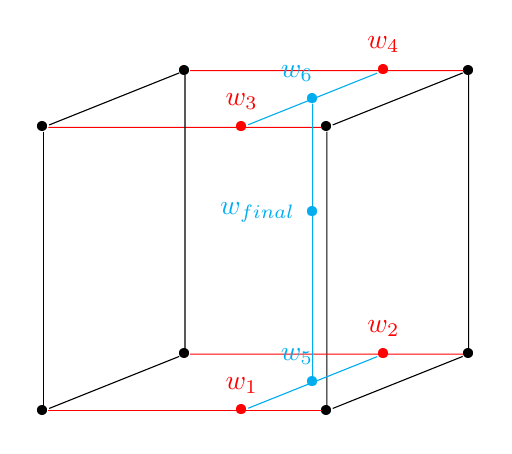
\begin{tikzpicture}[scale=1.8, x=2cm,y=2cm]
            \tikzset{c/.style = {shorten <=-4pt, shorten >=-4pt}}
            \tikzset{smalledge/.style = {-{Latex[length=2mm]},shorten <=-4pt}}
            
            \node (x1y1z1) at (0,0) {\small\textbullet};
            \node (x2y1z1) at (1,0) {\small\textbullet};
            \node (x1y2z1) at (0,1) {\small\textbullet};
            \node (x2y2z1) at (1,1) {\small\textbullet};
            \node (x1y1z2) at (0.5,0.2) {\small\textbullet};
            \node (x2y1z2) at (1.5,0.2) {\small\textbullet};
            \node (x1y2z2) at (0.5,1.2) {\small\textbullet};
            \node (x2y2z2) at (1.5,1.2) {\small\textbullet};
            
            \draw[c,red] (x1y1z1) -- (x2y1z1);
            \draw[c] (x2y1z1) -- (x2y2z1);
            \draw[c,red] (x2y2z1) -- (x1y2z1);
            \draw[c] (x1y2z1) -- (x1y1z1);

            \draw[c,red] (x1y1z2) -- (x2y1z2);
            \draw[c] (x2y1z2) -- (x2y2z2);
            \draw[c,red] (x2y2z2) -- (x1y2z2);
            \draw[c] (x1y2z2) -- (x1y1z2);

            \draw[c] (x1y1z1) -- (x1y1z2);
            \draw[c] (x1y2z1) -- (x1y2z2);
            \draw[c] (x2y1z1) -- (x2y1z2);
            \draw[c] (x2y2z1) -- (x2y2z2);

            % interpolations
            \node[red] (w1) at (0.7,0) {\textbullet};
            \node[red] (w2) at (1.2,0.2) {\textbullet};
            \node[red] (w3) at (0.7,1) {\textbullet};
            \node[red] (w4) at (1.2,1.2) {\textbullet};

            \draw[c,cyan] (w1) -- (w2);
            \draw[c,cyan] (w3) -- (w4);

            \node[cyan] (w5) at (0.95,0.1) {\textbullet};
            \node[cyan] (w6) at (0.95,1.1) {\textbullet};
            \node[cyan] (wfinal) at (0.95,0.7) {\textbullet};

            \draw[c,cyan] (w5) -- (w6);

            \draw[c, red] (w1) node[yshift=.1cm,above]{$w_1$};
            \draw[c, red] (w2) node[yshift=.1cm,above]{$w_2$};
            \draw[c, red] (w3) node[yshift=.1cm,above]{$w_3$};
            \draw[c, red] (w4) node[yshift=.1cm,above]{$w_4$};
            \draw[c, cyan] (w5) node[yshift=.1cm,xshift=-.2cm,above]{$w_5$};
            \draw[c, cyan] (w6) node[yshift=.1cm,xshift=-.2cm,above]{$w_6$};

            \draw[c, cyan] (wfinal) node[xshift=-.1cm,left]{$w_{final}$};

        \end{tikzpicture}
        \captionof{figure}{Perlin vertex weights in 3D space with eight corners and seven interpolations.}
        \label{img:tikz:noise:perlin:interpolation3d}    
    \end{minipage}
\end{figure}

\noindent
The amount of interpolations $i$ is therefore $i = 2^n-1$, where $n$ is the number of dimensions. As seen above, this gives $i = 3$ for 2D and $i = 7$ for 3D.

\begin{figure}[H]
    \centering
        \begin{minipage}{0.47\linewidth}
            \includegraphics[width=\linewidth]{noise/2D perlin unfaded}
            \captionof{figure}{2D Perlin noise texture with a 10x10 grid.}
            \label{img:noise:perlin:2d_unfaded}
        \end{minipage}
    \hfill
        \begin{minipage}{0.47\linewidth}
            \includegraphics[width=\linewidth]{noise/2D perlin}
            \captionof{figure}{2D Perlin noise texture with Perlin's fade function.}
            \label{img:noise:perlin:2d}
        \end{minipage}
\end{figure}

\noindent
By default, the perlin noise texture shows a significant amount of artifacts along the grid lines. This can be fixed by using Perlin's fade function \cite{online:perlin:impl} for $d_x$ and $d_y$, which is defined by $f(t) = 6t^5-15t^4+10t^3$.
\emptyline
For 3D, Perlin describes that rather than calculating random gradient vectors, a simple set of 12 distinct vectors can be used, which still provides sufficient randomness but is faster \cite{online:perlin:improved}.
For each grid corner, a hash function is used to generate an index (from 0 to 11), with which one of the gradient vectors is then chosen.


\clearpage
\subsubsection{Voronoi Noise}
While Perlin's noise algorithm is heavy on vector calculation and interpolation, other noise patterns are less complex to understand and construct, like the \textit{Voronoi} noise, also known as \textit{Worley} or \textit{cellular} noise.
The name derives from its similar structure to a Voronoi diagram, in which points, called \textit{seeds}, are randomly scattered inside a defined space. After that, regions are created, consisting of all points closer to that seed than to any other.
\emptyline
As for the noise pattern, there are some alterations. To get a more even distribution, the noise algorithm starts by dividing the space into a grid, for which each cell is assigned a random point. From there, each fragment gets colored by how far it is to the closest seed in its cell.

\begin{figure}[H]
    \centering

    \begin{minipage}{0.47\linewidth}
        \centering
        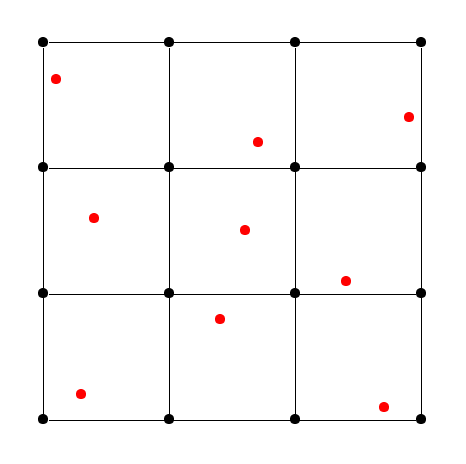
\begin{tikzpicture}[scale=0.8, x=2cm,y=2cm]
        \tikzset{c/.style = {shorten <=-4pt, shorten >=-4pt}}
        \tikzset{smalledge/.style = {-{Latex[length=2mm]},shorten <=-4pt}}
        
        \node (x1y1) at (0,0) {\textbullet};
        \node (x2y1) at (1,0) {\textbullet};
        \node (x3y1) at (2,0) {\textbullet};
        \node (x4y1) at (3,0) {\textbullet};

        \node (x1y2) at (0,1) {\textbullet};
        \node (x2y2) at (1,1) {\textbullet};
        \node (x3y2) at (2,1) {\textbullet};
        \node (x4y2) at (3,1) {\textbullet};

        \node (x1y3) at (0,2) {\textbullet};
        \node (x2y3) at (1,2) {\textbullet};
        \node (x3y3) at (2,2) {\textbullet};
        \node (x4y3) at (3,2) {\textbullet};

        \node (x1y4) at (0,3) {\textbullet};
        \node (x2y4) at (1,3) {\textbullet};
        \node (x3y4) at (2,3) {\textbullet};
        \node (x4y4) at (3,3) {\textbullet};

        \draw[c] (x1y1) edge node{} (x4y1);
        \draw[c] (x1y2) edge node{} (x4y2);
        \draw[c] (x1y3) edge node{} (x4y3);
        \draw[c] (x1y4) edge node{} (x4y4);

        \draw[c] (x1y1) edge node{} (x1y4);
        \draw[c] (x2y1) edge node{} (x2y4);
        \draw[c] (x3y1) edge node{} (x3y4);
        \draw[c] (x4y1) edge node{} (x4y4);

        \node[red] (s1) at (0.3,0.2) {\textbullet};
        \node[red] (s2) at (1.4,0.8) {\textbullet};
        \node[red] (s3) at (2.7,0.1) {\textbullet};
        \node[red] (s4) at (0.4,1.6) {\textbullet};
        \node[red] (s5) at (1.6,1.5) {\textbullet};
        \node[red] (s6) at (2.4,1.1) {\textbullet};
        \node[red] (s7) at (0.1,2.7) {\textbullet};
        \node[red] (s8) at (1.7,2.2) {\textbullet};
        \node[red] (s9) at (2.9,2.4) {\textbullet};

        \end{tikzpicture}
        \captionof{figure}{Voroni grid with pseudo-randomly assigned seed points for each cell.}
        \label{img:tikz:noise:voronoi}
    \end{minipage}
    \hfill
    \begin{minipage}{0.47\linewidth}
        \centering
        \begin{tikzpicture}[scale=0.8, x=2cm,y=2cm]
            \tikzset{c/.style = {shorten <=-4pt, shorten >=-4pt}}
            \tikzset{smalledge/.style = {-{Latex[length=2mm]},shorten <=-4pt}}
            
            \node (gradient) at (1.5,1.5) {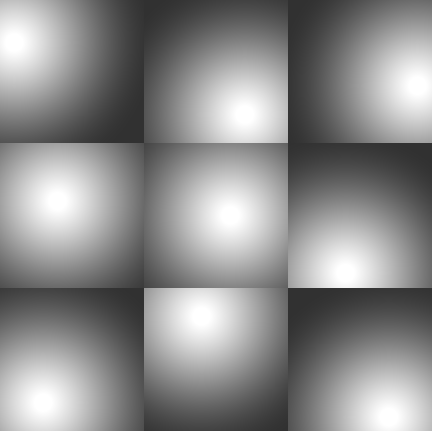
\includegraphics[width=4.8cm] {noise/2d voronoi unmixed}};

            \node (x1y1) at (0,0) {\textbullet};
            \node (x2y1) at (1,0) {\textbullet};
            \node (x3y1) at (2,0) {\textbullet};
            \node (x4y1) at (3,0) {\textbullet};

            \node (x1y2) at (0,1) {\textbullet};
            \node (x2y2) at (1,1) {\textbullet};
            \node (x3y2) at (2,1) {\textbullet};
            \node (x4y2) at (3,1) {\textbullet};

            \node (x1y3) at (0,2) {\textbullet};
            \node (x2y3) at (1,2) {\textbullet};
            \node (x3y3) at (2,2) {\textbullet};
            \node (x4y3) at (3,2) {\textbullet};

            \node (x1y4) at (0,3) {\textbullet};
            \node (x2y4) at (1,3) {\textbullet};
            \node (x3y4) at (2,3) {\textbullet};
            \node (x4y4) at (3,3) {\textbullet};

            \draw[c] (x1y1) edge node{} (x4y1);
            \draw[c] (x1y2) edge node{} (x4y2);
            \draw[c] (x1y3) edge node{} (x4y3);
            \draw[c] (x1y4) edge node{} (x4y4);

            \draw[c] (x1y1) edge node{} (x1y4);
            \draw[c] (x2y1) edge node{} (x2y4);
            \draw[c] (x3y1) edge node{} (x3y4);
            \draw[c] (x4y1) edge node{} (x4y4);

            \node[red] (s1) at (0.3,0.2) {\textbullet};
            \node[red] (s2) at (1.4,0.8) {\textbullet};
            \node[red] (s3) at (2.7,0.1) {\textbullet};
            \node[red] (s4) at (0.4,1.6) {\textbullet};
            \node[red] (s5) at (1.6,1.5) {\textbullet};
            \node[red] (s6) at (2.4,1.1) {\textbullet};
            \node[red] (s7) at (0.1,2.7) {\textbullet};
            \node[red] (s8) at (1.7,2.2) {\textbullet};
            \node[red] (s9) at (2.9,2.4) {\textbullet};

        \end{tikzpicture}
        \captionof{figure}{Voroni grid with seed distances visualized.}
        \label{img:tikz:noise:voronoi2}
    \end{minipage}
\end{figure}

\noindent
As understandable, in \autoref{img:tikz:noise:voronoi2}, hard contours are still visible along the grid lines. The final step is done by including the adjacent cells when finding the closest seed for any given fragment.
This amounts to $3^n - 1$ neightboring cells, where $n$ is the number of dimensions. This means for 2D space its eight cells, while in 3D its 26.

\begin{figure}[H]
    \centering
    \begin{tikzpicture}[scale=1.2, x=2cm,y=2cm]
        \tikzset{c/.style = {shorten <=-4pt, shorten >=-4pt}}
        \tikzset{smalledge/.style = {-{Latex[length=2mm]},shorten <=-4pt}}
        
        \node (gradient) at (1.5,1.5) {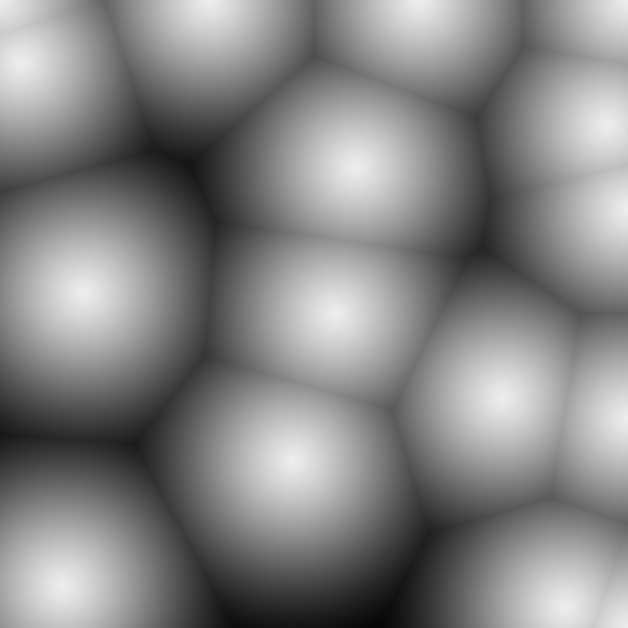
\includegraphics[width=7.2cm] {noise/2d voronoi}};

        \node (x1y1) at (0,0) {\textbullet};
        \node (x2y1) at (1,0) {\textbullet};
        \node (x3y1) at (2,0) {\textbullet};
        \node (x4y1) at (3,0) {\textbullet};

        \node (x1y2) at (0,1) {\textbullet};
        \node (x2y2) at (1,1) {\textbullet};
        \node (x3y2) at (2,1) {\textbullet};
        \node (x4y2) at (3,1) {\textbullet};

        \node (x1y3) at (0,2) {\textbullet};
        \node (x2y3) at (1,2) {\textbullet};
        \node (x3y3) at (2,2) {\textbullet};
        \node (x4y3) at (3,2) {\textbullet};

        \node (x1y4) at (0,3) {\textbullet};
        \node (x2y4) at (1,3) {\textbullet};
        \node (x3y4) at (2,3) {\textbullet};
        \node (x4y4) at (3,3) {\textbullet};

        \draw[c] (x1y1) edge node{} (x4y1);
        \draw[c] (x1y2) edge node{} (x4y2);
        \draw[c] (x1y3) edge node{} (x4y3);
        \draw[c] (x1y4) edge node{} (x4y4);

        \draw[c] (x1y1) edge node{} (x1y4);
        \draw[c] (x2y1) edge node{} (x2y4);
        \draw[c] (x3y1) edge node{} (x3y4);
        \draw[c] (x4y1) edge node{} (x4y4);

        \node[red] (s1) at (0.3,0.2) {\textbullet};
        \node[red] (s2) at (1.4,0.8) {\textbullet};
        \node[red] (s3) at (2.7,0.1) {\textbullet};
        \node[red] (s4) at (0.4,1.6) {\textbullet};
        \node[red] (s5) at (1.6,1.5) {\textbullet};
        \node[red] (s6) at (2.4,1.1) {\textbullet};
        \node[red] (s7) at (0.1,2.7) {\textbullet};
        \node[red] (s8) at (1.7,2.2) {\textbullet};
        \node[red] (s9) at (2.9,2.4) {\textbullet};

    \end{tikzpicture}
    \captionof{figure}{Complete 2D Voroni noise pattern.}
    \label{img:tikz:noise:voronoi3}
\end{figure}

\noindent
An implementation of this relatively simple algorithm could look like the following listing. In it, \lstinline[language=HLSL]{randomSeed()} is used like the previously introduced function \lstinline[language=HLSL]{random()}, except that it returns a two-dimensional vector instead of a scalar.
With that, a deterministically random point can be generated for any given cell.

\begin{lstlisting}[language=HLSL, caption=Implementation of 2D Voronoi noise algorithm., label=lst:shader:noise:voronoi2d]
float2 randomSeed(float2 co) {
    return float2(
        fract(sin(dot(co, float2(12.9898, 78.233))) * 43758.5453123),
        fract(sin(dot(co, float2(39.3461, 11.135))) * 14375.8545359));
}

float voronoi(float2 p) {
    float2 pCell = floor(p);
    float dMin = 999;

    for(int x = -1; x <= 1; x++) {
        for(int y = -1; y <= 1; y++) {
            float2 cell = pCell + float2(x, y);
            float2 seed = cell + randomSeed(cell);
            float d = distance(seed, p);
            if (d < dMin) {
                dMin = d;
            }
        }
    }
    
    return dMin;
}
\end{lstlisting}

\noindent
Since the Voronoi noise algorithm creates a cellular pattern, it is well suitable for simulating natural distribution of cloud heaps, as they are in some way also formed "in cells". 

\clearpage
\subsubsection{Fractal Brownian Motion}
In the world of shaders, the term \textit{fractal Brownian motion} (fBm) is often described as adding different levels of noise together, thus creating a self-similar pattern across different scales \cite{online:thebookofshaders:fractal}.
This simplified description meets the required level of detail for this section, a complete explanation and derivation of the fractal Brownian motion is beyond the scope of this paper.
\emptyline
In shaders, fBms are also called \textit{fractal noise}. They are usually implemented by adding different iterations of noise (called \textit{octaves}), while successively incrementing the frequencies in regular steps (\textit{lacunarity}) and decreasing the amplitude (\textit{gain}) of the noise.
This results in a more detailed noise, meaning a finer granularity of the  pattern in the noise.

\begin{lstlisting}[language=HLSL, caption=Implementation of fractal Brownian motion function., label=lst:shader:fbm]
#define LACUNARITY 2.0
#define GAIN 0.5
#define OCTAVES 1
    
float fbm(float2 p) {
    float frequency = 1.0;
    float amplitude = 0.5;
    
    float total = 0;
    float maxValue = 0;
    for(int i = 0; i < OCTAVES; i++) {
        float current = noise(p * frequency) * amplitude;
        total += current;
        maxValue += amplitude;
        
        amplitude *= GAIN;
        frequency *= LACUNARITY;
    }
    
    return total/maxValue;
}
\end{lstlisting}

\noindent
Interestingly, the only things that change for 3D is \lstinline[language=HLSL]{float2 p} becomes a \lstinline[language=HLSL]{float3 p} and the \lstinline[language=HLSL]{noise()} function must accept a three-dimensional vector instead. That's all.
\\
Here are some example images of the fractal Brownian motion with different octaves. For the noise function, a Voronoi noise algorithm was used.
\begin{figure}[H]
    \centering
        \begin{minipage}{0.3\linewidth}
            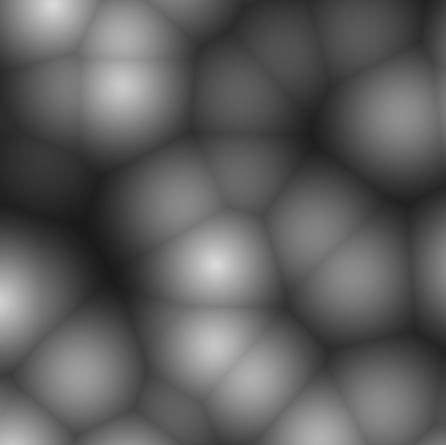
\includegraphics[width=\linewidth]{noise/fbm1}
            \captionof{figure}{One octave of a 2D Voronoi noise.}
            \label{img:noise:fbm1}
        \end{minipage}
        \hfill
        \begin{minipage}{0.3\linewidth}
            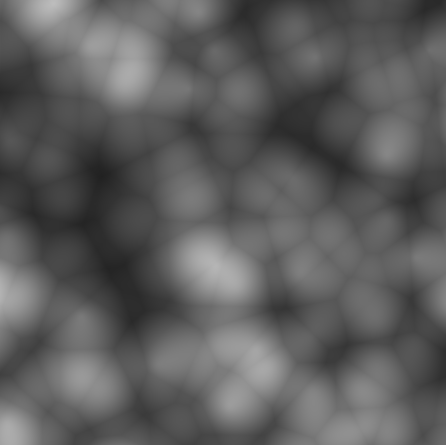
\includegraphics[width=\linewidth]{noise/fbm2}
            \captionof{figure}{Two octaves of a 2D Voronoi noise.}
            \label{img:noise:fbm2}
            \end{minipage}
        \hfill
        \begin{minipage}{0.3\linewidth}
            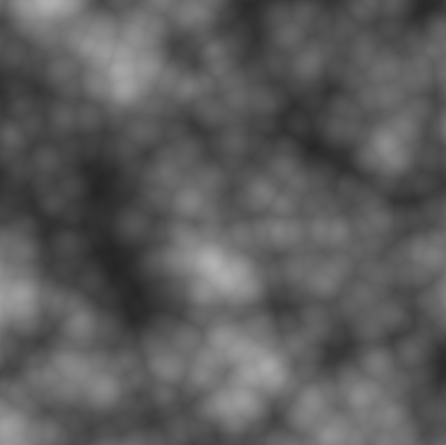
\includegraphics[width=\linewidth]{noise/fbm3}
            \captionof{figure}{Three octaves of a 2D Voronoi noise.}
            \label{img:noise:fbm6}
        \end{minipage}
\end{figure}

\noindent
It is understandable that with every additional octave, the algorithm has to evaluate the noise at the given point again, making it worth considering the impact on performance fractal noise has.
However, the final renders look convincingly "cloudy".

\begin{figure}[H]
    \centering
        \begin{minipage}{0.47\linewidth}
            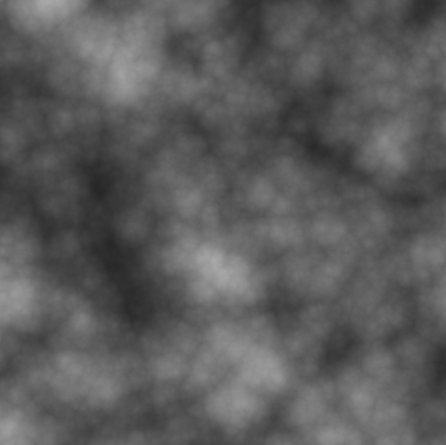
\includegraphics[width=\linewidth]{noise/fbm10_1}
            \captionof{figure}{Ten octaves of a 2D Voronoi noise.}
            \label{img:noise:fbm10_1}
        \end{minipage}
    \hfill
        \begin{minipage}{0.47\linewidth}
            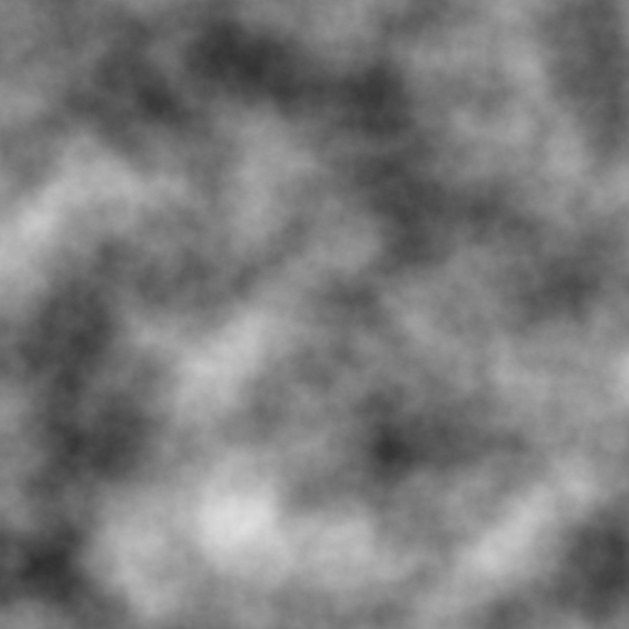
\includegraphics[width=\linewidth]{noise/fbm10_2}
            \captionof{figure}{Ten octaves of a 2D Perlin noise.}
            \label{img:noise:fbm10_2}
        \end{minipage}
\end{figure}